\chapter{Обзор методов обучения с подкреплением и их применения в роботике}\label{ch:ch1}

В настоящее время вычислительные технологии достигли выдающихся результатов. Так обычный процессор спослобен производить до $10^8$ операций в секунду. Однако до недавнего времени компьютер существенно проигрывал человеку в решении сложно формализцемых задач таких как распознавание изображений и анализ текстов на естественном языке. 

Существенный перелом наступил в 2010 году когда с помощью нейронной сети AlexNet было достигнуто качество классификации изображений превосходящее человека. TODO рассказать про посдедующие улучшения, Рассказать про imagenet.
Также в анализе естественного языка был достигнут большой прогресс основанный на применении глубоких нейронных сетей таких как bert. В случае обработки изображений используются наборы данных размеченные человеком. В случае обработки текстов используются не структурированные данные в которых нейронная сеть учится предсказывать следующее слово исходя из контекста. 

Важным подходом для создания общего искусственного интеллекта является обучение с подкреплением \cite{reward_is_enough}. Оно наиболее похоже на то, как обучаются и исследуют мир люди и животные.  


\section{Обзор методов глубокого обучения с подкреплением}\label{sec:ch1/sec1}

Глубокое обучение с подкреплением основанно на объединении глубоких нейронных сетей и методов обучения с подкреплением. 
В основном они делятся на два класса 

\subsection{Нейронные сети}

Первая нейронная сеть была предложена Фрэнком Розенблаттом в 1957 году \cite{rosenblatt}. Это была нейронная сеть с одним скрытым слоем, пороговой функцией активации и прямым распространением сигнала. 


Нейронная сеть как универсальный аппроксиматор
Теорема колмогорова


\subsection{Обучение с подкреплением}

Принципиальная схема обучения RL алгоритмов приведена на рисунке \ref{fig:rl}. На ней агент получает от среды состояние (s $\in \mathcal{R}^n$), награду (reward $\in \mathcal{R}^1$), и флаг завершения эпизода (done $\in \{0, 1\}$).  В среде агент совершает действие (action $\in \mathcal{R}^m$) которое переводит среду в следующее состояние (s' $\in \mathcal{R}^n$). В зависимости от того является ли переход из состояния $s$ в состояние $s'$ при действии $a$ единственным или одним из возможных с вероятностью $p(s',r|s,a)$, среда называется детерменированной или не детерменированной. 

\begin{figure}[ht]
	\centerfloat{
		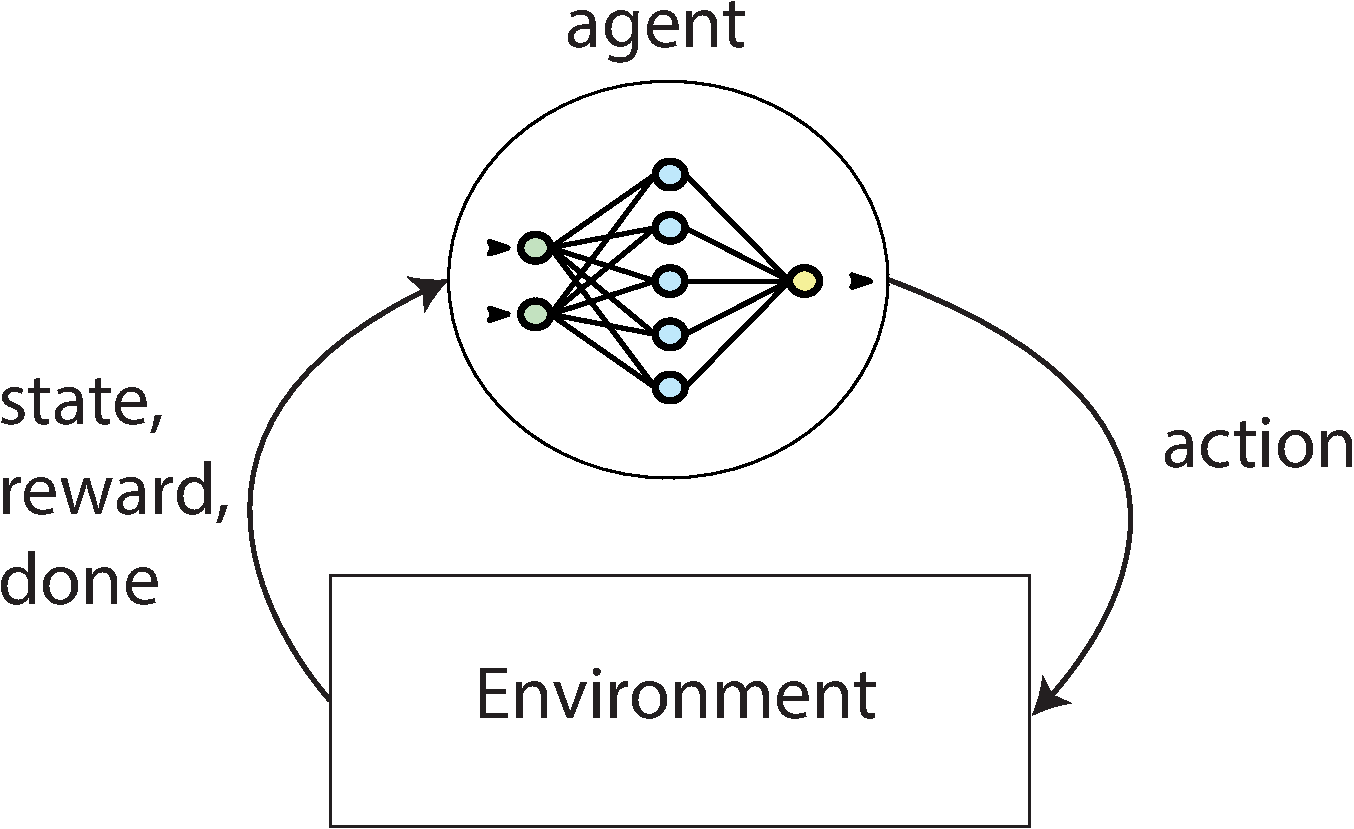
\includegraphics[width=0.5\linewidth]{images/rl_setting}
	}
	\caption{Взаимодействие агента и среды}
	\label{fig:rl}
\end{figure}

Процесс работы RL агента строится на марковском прецессе принтия решений (МППР). В нем предполагается, что следующее состояние и награда которую получит агент зависит только от предыдуюего состояния и действия которое агент совершил (не дет среды?). Если же у среды есть некоторые не наблюдаемые параметры, то говорят о частично наблюдаемом марковском процессе принятия решений (ЧНМППР). 

Задача агента состоит в максимизации суммарной ожидаемой дисконтированной награды к конецу эпизода:

\begin{equation}
E_{\tau \sim \pi(\theta)} [G(\tau)] = E_{\tau \sim \pi(\theta)} [R_0 + \gamma R_{1} + \gamma ^ 2 R_{2} + ...] = E_{\tau \sim \pi(\theta)} [\sum_{t=0}^{T - 1} \gamma ^t R_{t}]
\end{equation}

Коэффициент $\gamma \in (0, 1]$ вводится для эффективного ограничения горизонта (пояснить) и он позволяет регулировать уровень жадности агента: на сколько награда получаемая на текущем шаге ценнее агалогичной награды получаемой на следующем шаге.  


\subsection{Уравнение Беллмана}

Для того, чтобы оценить ценность состояния вводятся V, Q-функции. (рассказать про динамической программирование, привести пример с сеткой и роботом идущим из верхнего угла в нижний). 

\begin{equation}
	V^*(s) = \max_{a \in \mathcal{A}} E(r_{t + 1} + \gamma V^*(s_{t + 1}))
\end{equation}

\begin{equation}
Q^*(s, a) = E(r_{t + 1} + \gamma \max_{a' \in \mathcal{A}} Q^*(s_{t + 1}, a'))
\end{equation}
 
\subsection{Value iteration}

Применение метода простой инерации к уравнению Беллмана. Данный метод доказано сходится (дать ссылку на Саттона?) однако в нем трубется конечное количество состояний среды и известные вероятности переходов и наград. 

\begin{algorithm}[H]
	\SetAlgoLined
	\KwResult{Write here the result }
	\KwOut{$\pi(s) = argmax_{a} \sum_{s', r}p(s',r|s,a)[r + \gamma V(s')]$}
	initialization V(s) = 0 (for all $s \in \mathcal{S}$)\;
	\While{$\Delta$ > threshold}{
		$\Delta$ = 0\;
		\ForEach{s $\in \mathcal{S}$}{
			V(s) = $\max_a \sum_{s', r}p(s', r|s, a)[r + \gamma V(s')]$
		}
	}
	\caption{Value iteration algorithm}
\end{algorithm}

\subsection{Policy iteration}
Что это 
Доказательство сходимости

\begin{algorithm}[H]
	\SetAlgoLined
	\KwResult{Write here the result }
	\KwOut{$\pi(s) = argmax_{a} \sum_{s', r}p(s',r|s,a)[r + \gamma V(s')]$}
	initialization V(s) = 0 (for all $s \in \mathcal{S}$)\;
	\While{$\Delta$ > threshold}{
		$\Delta$ = 0\;
		\ForEach{s $\in \mathcal{S}$}{
			$\pi(s) = argmax_{a}Q(s,a)$
		}
	}
	\caption{Policy iteration algorithm}
\end{algorithm}

\subsection{Q-learing}
Что это
Пример с табличкой
гамма
метод временных разностей, адвантаж, оверэстимэйшен 
DQN, DDPG, TD3, SAC

\subsection{Policy gradient}
credit assignment problem (какие действия привели к награде)
Альтернативным подходом является оптимизация стратегии на прямую. 

$$J(s) = \sum_{\pi} R(s,a )$$
$$\nabla_{\theta} J(s) = \sum_{\pi} \pi(a|s)\frac{\nabla \pi(a|s)}{\pi(a|s)}R(s,a )$$
$$\nabla_{\theta} J(s) = \sum \log(\pi(a|s))R(s,a )$$

Мотивация 
REINFORCE, Actor-Critic, PPO

\subsection{Meta-learning}
Мотивация MAML, PEARL, RL2

\section{Обзор применения методов обучения с подкреплением в роботике}\label{sec:ch1/sec2}
Перечислить подходы и открытые проблемы (from proposal)


\section{Ссылки}\label{sec:ch1/sec2}


\FloatBarrier
